
\documentclass[12pt]{article}
\usepackage[spanish]{babel}
\usepackage[utf8]{inputenc}
\usepackage{amsmath}
\usepackage{graphicx}
\usepackage{geometry}
\geometry{margin=2.5cm}
\usepackage{graphicx}
\usepackage{subcaption}

\title{Efecto de la sincronización en el proceso de aprendizaje de una red neuronal}
\author{Laura Ximena Rodriguez Quintero}
\date{22 de junio de 2025}

\begin{document}
\maketitle

\begin{abstract}
Los sistemas complejos exhiben transiciones de fase en las que pasan de estados desordenados a estados ordenados cuando un parámetro de control supera un umbral crítico. Un caso paradigmático es la sincronización de osciladores: por debajo del acoplamiento crítico las fases permanecen incoherentes y, al superarlo, emerge sincronía global, fenómeno que el modelo de Kuramoto describe de forma canónica \cite{Kuramoto1984,Strogatz2000}. En este trabajo estudiamos cómo estas transiciones de sincronización afectan el aprendizaje cuando las unidades de la red son osciladores acoplados que evolucionan según la dinámica de Kuramoto, implementados en el marco de \textit{Artificial Kuramoto Oscillatory Neurons} (AKOrN) \cite{Miyato2024}. Mostramos que, al barrer parámetros de acoplamiento, la red atraviesa un cambio cualitativo en su organización (de incoherente a parcialmente sincronizada) y que operar cerca de dicho punto crítico se asocia con correlaciones de largo alcance y un comportamiento computacionalmente ventajoso, en línea con la literatura sobre criticalidad neuronal \cite{Breakspear2010,ShewPlenz2013,Myrov2024}. Estos resultados conectan la física de sistemas fuera del equilibrio con el diseño de arquitecturas de aprendizaje que explotan sincronización para crear representaciones robustas.

\textit{Palabras clave:} sincronización, criticalidad, transiciones de fase, Kuramoto, AKOrN, redes neuronales.
\end{abstract}

\section{Introducción}

Los cambios de fase de desorden a orden son un rasgo de la física estadística: una variación suave de un parámetro externo puede inducir un cambio cualitativo en el comportamiento colectivo de un sistema. En poblaciones de osciladores de fase, el modelo de Kuramoto predice una transición continua (de segundo orden) entre un régimen incoherente y otro sincronizado cuando el acoplamiento supera un umbral crítico \cite{Kuramoto1984,Strogatz2000}. Cerca de ese punto crítico emergen correlaciones de largo alcance y fluctuaciones sin escala que se han propuesto como rasgos funcionales en el cerebro, donde operar “al borde de la criticidad” puede maximizar rango dinámico y transmisión de información \cite{ShewPlenz2013}.

Motivados por estas observaciones, adoptamos el modelo \textit{Artificial Kuramoto Oscillatory Neurons} (AKOrN) como bloque dinámico en redes neuronales. En AKOrN, cada unidad es un oscilador cuya fase evoluciona bajo acoplamientos locales y entradas externas; la pila de capas aplica la actualización de Kuramoto durante varias iteraciones y un módulo de lectura genera estímulos para la siguiente capa. Esta construcción permite usar conectividades convolucionales (locales) o de atención (dinámicas), manteniendo compatibilidad con arquitecturas profundas modernas \cite{Miyato2024}. En paralelo, nos apoyamos en hallazgos recientes de modelado cerebral que relacionan la sincronización crítica con la aparición de correlaciones temporales de largo alcance (p. ej., exponentes DFA elevados) \cite{Myrov2024}. 

A lo largo de este trabajo, exploramos cómo la red transita de estados desincronizados a estados parcialmente sincronizados al variar el acoplamiento y cómo esa cercanía a la transición crítica se refleja en métricas dinámicas (parámetro de orden, espectros 1/f, DFA) y en el rendimiento de aprendizaje. Esta perspectiva integra principios de sistemas complejos con el diseño de redes neuronales.

La sincronización es un fenómeno en el cual diversas partes de un mismo sistema comparten una misma dinámica. Como consecuencia, emergen patrones coherentes en el sistema y estos dependen de la forma en la que cada una de las partes interacciona. Podemos llegar a entender estos comportamientos como  arreglos de osciladores acoplados entre si, donde las propiedades de la sincronización depende de las formas de acoplamiento. En general, la sincronización puede ser descrita mediante la ecuación (\ref{basica}), donde cada $\{\phi\}$ representa el conjunto de todos los $\phi_{i}$. Aquí se observa que la evolución de cada una de las partes del sistema depende de la forma en la que este interacciona con los demás elementos. 
\begin{equation}
    \frac{d\phi_{i}}{dt}= f_{i}(\{\phi\})
    \label{basica}
\end{equation}


Para describir la sincronización de forma más precisa, utilizamos el modelo de  Yoshiki Kuramoto propuesto en 1984\cite{Kuramoto1984}. Este modelo, dependiendo de las dinámicas, tiene diferenes formas, pero en escencia es la misma idea, la evolución temporal de la fase depende de las diferencias entre las fases con los vecinos más cercanos. Una de esas variantes corresponde a la ecuación (\ref{eq:kuramoto}), aquí debemos considerar un ensamble de osciladores acoplados según  los elementos de matriz $J_{ij}$, la frecuencia natural de oscilación $\omega_{i}$ y la diferencia de fase entre los osciladores. 

\begin{equation} 
\dot{\theta_{i}}= \omega_{i} + \sum_jJ_{ij}\sin(\theta_j - \theta_i)
\label{eq:kuramoto}
\end{equation}

Así pues, el modelo de Kuramoto nos permite cuantificar la sincronización de los sistemmas mediantes el parámetro de orde $r(t)$ (ecuación \ref{parametro r}) . Este parámetro varia entre $0$ y $1$, representando un sistema completamente desincronizado o completamente sincronizado respectivamente. También puede entender como una medida del movimiento colectivo producido por un grupo de N osciladores en el plano complejo, con $\theta(t)$ la fase promedio de los rotores .


\begin{equation}
r(t)= \left| \frac{1}{N} \sum _{j=1}^{N} e ^{i\theta(t)_{j}} \right|
    \label{parametro r}
\end{equation}

La sincronización emerge en sistemas tanto naturales como artificiales, manifestándose en procesos tan diversos como terremotos, ecosistemas, actividad neuronal, marcapasos, células, comportamientos animales o sistemas de resortes, entre otros. Se ha demostrado que la sincronización juega un papel fundamental en redes de aprendizaje, tanto en el cerebro como en redes neuronales artificiales, especialmente en aquellas inspiradas en principios biológicos. En el cerebro, la sincronización se manifiesta en patrones de actividad colectiva de millones de neuronas, como las avalanchas neuronales y los ritmos oscilatorios. En redes neuronales artificiales, las Artificial Kuramoto Oscillatory Neurons (AKOrN) se inspiran en este modelo biológico y utilizan la sincronización como un mecanismo de procesamiento de la información. \\

La principal característica de AKOrN es la simulación del binding observado en neurociencia, un mecanismo que permite comprimir representaciones mediante la sincronización. Este fenómeno es crucial para integrar información distribuida y generar representaciones coherentes. \\

En síntesis, el problema central radica en entender cómo la sincronización emerge de manera autoorganizada en sistemas complejos y caóticos para facilitar el aprendizaje y un comportamiento flexible, y cómo estos principios pueden replicarse y controlarse en sistemas artificiales. Comprender el por qué y el cómo de esta autoorganización es clave para desentrañar los mecanismos del aprendizaje en el cerebro y diseñar redes neuronales artificiales más potentes y biológicamente plausibles. \\

A medida que ampliamos nuestra comprensión del cerebro, descubrimos más sobre los principios de procesamiento de la información y su relación con la sincronización, principios que pueden ser aplicados en las arquitecturas de redes neuronales. En este contexto, este trabajo se propone explorar la relación entre sincronización y aprendizaje en una red neuronal cuyas unidades fundamentales de procesamiento corresponden a resortes acoplados que evolucionan de acuerdo con las dinámicas del modelo de Kuramoto.


\section{Metodología}

En esta sección se describe el procedimiento seguido para estudiar la relación entre sincronización y aprendizaje en la red neuronal basada en el modelo de Kuramoto. La metodología se estructura en tres etapas principales: (i) construcción del modelo dinámico y cálculo del parámetro de orden, (ii) caracterización estadística de la sincronización y de la transición de fase en función del acoplamiento externo, y (iii) entrenamiento y evaluación de la red neuronal con y sin el bloque AKOrN.

\subsection{Modelo de Kuramoto y parámetro de orden}

En primer lugar, se modeló cada imagen del conjunto de datos MNIST como un sistema de osciladores acoplados que evolucionan según la ecuación de Kuramoto (ecuación~\ref{eq:kuramoto}). A cada píxel se le asoció un oscilador con fase \(\theta_i(t)\), frecuencia natural \(\omega_i\) y acoplamientos \(J_{ij}\) definidos a partir de la conectividad local de la imagen (vecindad espacial). La intensidad de la entrada externa se parametrizó mediante una constante de acoplamiento global \(c\), que controla la fuerza con la que la dinámica tiende a sincronizarse.

Para cuantificar el grado de sincronización global se utilizó el parámetro de orden de Kuramoto \(r(t)\) definido en la ecuación~\ref{parametro r}. Para cada imagen se integró numéricamente la dinámica desde condiciones iniciales aleatorias hasta un tiempo final \(T\), y se calculó el valor estacionario del parámetro de orden, \(R = r(T)\), así como la trayectoria temporal \(r(t)\). Este procedimiento se repitió para un barrido de valores de \(c\) en un intervalo \([0, c_{\max}]\), obteniendo así curvas \(R(c)\) individuales por imagen.

\subsection{Distribuciones de sincronización y transición de fase}

Con el fin de caracterizar estadísticamente el régimen estacionario de la dinámica, se calcularon las distribuciones del parámetro de orden estacionario \(R\) para todo el conjunto de datos y por clase (dígito). A partir de las curvas \(R(c)\) se identificó, para cada imagen, un valor crítico de acoplamiento \(c_{\text{crítico}}\) asociado al punto en el que el sistema pasa de un régimen desincronizado (\(R \approx 0\)) a un régimen sincronizado (\(R > 0\)). El valor de \(R\) en ese punto se definió como \(R_{\text{crítico}}\).

Para estudiar la transición de fase promedio, se construyeron curvas \(\langle R(c) \rangle\) promediando el parámetro de orden sobre todas las imágenes de la base de datos para cada valor de \(c\). Estas curvas permitieron identificar el intervalo de acoplamiento en el que la sincronización emerge de forma colectiva y cuantificar el régimen de sincronización parcial. Asimismo, se generaron distribuciones de \(R_{\text{crítico}}\) y \(c_{\text{crítico}}\) por clase, con el objetivo de analizar cómo la geometría de los dígitos influye en la respuesta dinámica del sistema de osciladores.

Los cálculos numéricos de la dinámica de Kuramoto y el procesamiento estadístico (histogramas, estimaciones de densidad y promedios por clase) se implementaron en Python utilizando librerías científicas estándar (NumPy, SciPy, Matplotlib) y PyTorch para manejar de forma eficiente grandes volúmenes de datos. Los resultados se almacenaron en bases de datos SQLite (\texttt{.db}) y archivos binarios de métricas (\texttt{.pt}) que luego se emplearon para la generación de las figuras presentadas en la sección de Resultados.

\subsubsection{Arquitectura del código e implementación computacional}

La implementación completa del análisis se organizó en el directorio \texttt{Codigo\_final}, estructurado en tres módulos autocontenidos que reflejan las etapas metodológicas descritas:

\begin{enumerate}
    \item \textbf{Generación de métricas Kuramoto} (\texttt{analisis\_distribuciones/}):
     El script \\
     \texttt{generar\_metricas\_kuramoto\_train.py} procesa las 60,000 imágenes del conjunto de entrenamiento MNIST, integrando la dinámica de Kuramoto para cada una y almacenando la serie temporal completa del parámetro de orden \(r(t)\), así como otras métricas. Los resultados se guardan en \texttt{metricas\_completas\_TRAIN\_MAC\_60k.pt}.
     
    %  El script de análisis \texttt{plot\_distribuciones\_R\_stationary.py} genera las distribuciones del parámetro de orden estacionario \(R\) para todo el conjunto de datos y por clase.

    \item \textbf{Caracterización de criticalidad} (\texttt{analisis\_alpha\_c/}): Los scripts\\ \texttt{generar\_c\_critico\_mnist.py} y \texttt{generar\_R\_critico\_mnist.py} implementan el barrido de la constante de acoplamiento \(c\) para cada imagen, identificando los valores críticos \(c_{\text{crítico}}\) y \(R_{\text{crítico}}\) asociados a la transición de fase. Los resultados se almacenan en bases de datos SQLite organizadas por clase (\texttt{mnist\_c\_critical.db}, \texttt{mnist\_R\_critico.db}).

    \item \textbf{Análisis de transición de fase} (\texttt{analisis\_RvsC/}): El script\\ \texttt{generar\_curvas\_R\_vs\_C.py} calcula las curvas completas \(R(c)\) para cada imagen en el intervalo \([0, 0.4]\), guardando los resultados en \texttt{R\_vs\_C.db}. 
\end{enumerate}

\textbf{Componentes centrales de la arquitectura:} La implementación de la dinámica de Kuramoto se basa en dos clases principales definidas en el módulo \texttt{kuramoto.modelo}:

\begin{itemize}
    \item \textbf{Clase \texttt{KConv2d}} (\emph{capa convolucional de Kuramoto}): Representa la conectividad espacial entre osciladores mediante una convolución 2D que define la matriz de acoplamientos \(J_{ij}\). Esta clase implementa la ecuación de evolución del sistema:
    \[
    \dot{\mathbf{x}}_i = \boldsymbol{\Omega}_i \mathbf{x}_i + \text{Proj}_{\mathbf{x}_i^\perp} \left( \mathbf{c}_i + \sum_j \mathbf{J}_{ij} \mathbf{x}_j \right)
    \]
    donde \(\boldsymbol{\Omega}_i\) es la matriz antisimétrica que codifica la frecuencia natural de oscilación, \(\mathbf{x}_i\) representa el estado del oscilador en el píxel \(i\), \(\mathbf{c}_i\) es el campo de acoplamiento externo (modulado por la constante \(c\)), y la proyección ortogonal \(\text{Proj}_{\mathbf{x}_i^\perp}\) garantiza la conservación de la norma unitaria de los osciladores. Adicionalmente, la clase calcula la función de energía de Lyapunov:
    \[
    E = -\sum_{i,j} \mathbf{x}_i^T \mathbf{J}_{ij} \mathbf{x}_j - \sum_i \mathbf{c}_i^T \mathbf{x}_i
    \]
    que permite verificar la convergencia de la dinámica hacia estados estacionarios de mínima energía.

    \item \textbf{Clase \texttt{KBlock}} (\emph{bloque dinámico de Kuramoto}): Implementa la integración numérica de la ecuación diferencial mediante el método de Euler explícito con proyección de normalización en cada paso:
    \[
    \mathbf{x}_i^{(t+1)} = \Pi \left[ \mathbf{x}_i^{(t)} + \gamma \Delta t \, \Delta \mathbf{x}_i^{(t)} \right]
    \]
    donde \(\Pi[\cdot]\) denota la proyección a la esfera unitaria, \(\gamma\) es el factor de acoplamiento (típicamente \(\gamma = 0.7\)), y \(\Delta t\) es el paso temporal (\(\Delta t = 0.9\)). El método \texttt{forward} de esta clase ejecuta \(T\) pasos de integración (con \(T = 30\) para análisis de criticalidad y \(T = 100\) para generación de métricas completas) y permite registrar opcionalmente la serie temporal completa de estados \(\{\mathbf{x}(t)\}_{t=0}^T\) y las energías \(\{E(t)\}_{t=0}^T\), necesarias para calcular el parámetro de orden \(r(t)\) y analizar la evolución hacia el régimen estacionario.
\end{itemize}

Esta arquitectura modular permite separar claramente la simulación de la dinámica física (clases \texttt{KConv2d} y \texttt{KBlock}), el cálculo de métricas estadísticas (módulo \texttt{analisis.criticalidad}), y la generación de visualizaciones, garantizando reproducibilidad completa de los resultados presentados en este trabajo.

\subsection{Entrenamiento de la red neuronal con AKOrN}

En la última etapa, se integró la dinámica de Kuramoto en una arquitectura de red neuronal convolucional mediante el bloque AKOrN (Artificial Kuramoto Oscillatory Neurons). Este bloque actúa como una capa intermedia que recibe mapas de activación de una red convolucional estándar y los transforma en representaciones oscilatorias acopladas, cuya sincronización codifica información relevante para la tarea de clasificación.

Se entrenaron dos modelos sobre el conjunto de datos MNIST: (i) una red convolucional base sin AKOrN, y (ii) una red equivalente que incorpora el bloque AKOrN entre las capas convolucionales y las capas finales de clasificación. Ambos modelos se entrenaron bajo las mismas condiciones (número de épocas, tamaño de lote, tasa de aprendizaje y partición de entrenamiento/prueba) con el fin de comparar de forma justa su desempeño.

Durante el entrenamiento se registraron la función de pérdida y la precisión (\emph{accuracy}) tanto en el conjunto de entrenamiento como en el de prueba. En particular, se analizó la evolución del accuracy a lo largo de los test y se compararon las tasas de cambio de dicha métrica en los modelos con y sin AKOrN. Esta comparación permite evaluar cuantitativamente el efecto de incorporar sincronización oscilatoria en la arquitectura sobre la eficiencia y la calidad del aprendizaje supervisado.

En conjunto, estas tres etapas metodológicas —simulación de la dinámica de Kuramoto, análisis estadístico de la sincronización y evaluación comparativa del entrenamiento con AKOrN— proporcionan un marco coherente para explorar el papel de la sincronización en el procesamiento de información y en el rendimiento de redes neuronales inspiradas en sistemas físicos acoplados.



\section{Resultados}%%%%%%%%%%%%%%%%%55-----------------------
El tiempo de entrenamiento para una red que implementa AKOrN es de aproximadamente
1min, mientras que para una arquitectura sin AKOrN con dos capas convoluciones el tiempo
de entranmiento es de 30s aproximadamente, pero el modelo que incluye a AKOrN presenta
un mejor rendimiento según el accuracy, esto lo podemos observar en la figura 8. \\


%Comparación red normal y kuramoto
\begin{figure}[h!]
    \centering
    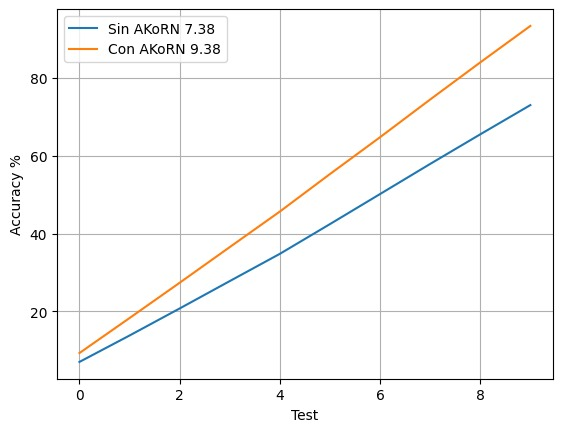
\includegraphics[width=0.6\linewidth]{akorn vs sin akorn.jpeg}
    \caption{Comparación en la exactitud durante el test para el modelo con AKOrN (naranja) y sin AKOrN (azúl) con sus respectivas tasas de cambio.}
    \label{fig:akorn vs sin akorn}
\end{figure}

En la figura \ref{fig:akorn vs sin akorn} vemos la evolución del porcentaje de precisión del modelo (Accu-
racy) respecto a cada uno de los test evaluados. La diferencia entre sus pendientes es de 2 unidades en cada evolución, es decir, por cada test que se realice para el modelo con AKOrN
la tasa de cambio es de $9,38$ y para el modelo sin AKOrN es de $7,38$. Con AKOrN la red alcanza un accuracy mayor al $90 \%$ con un entrenamiendo de 10 epoch para 60.000 datos de
entrenamiento y 10.000 de prueba. \\

\begin{figure}[h!]
    \centering
    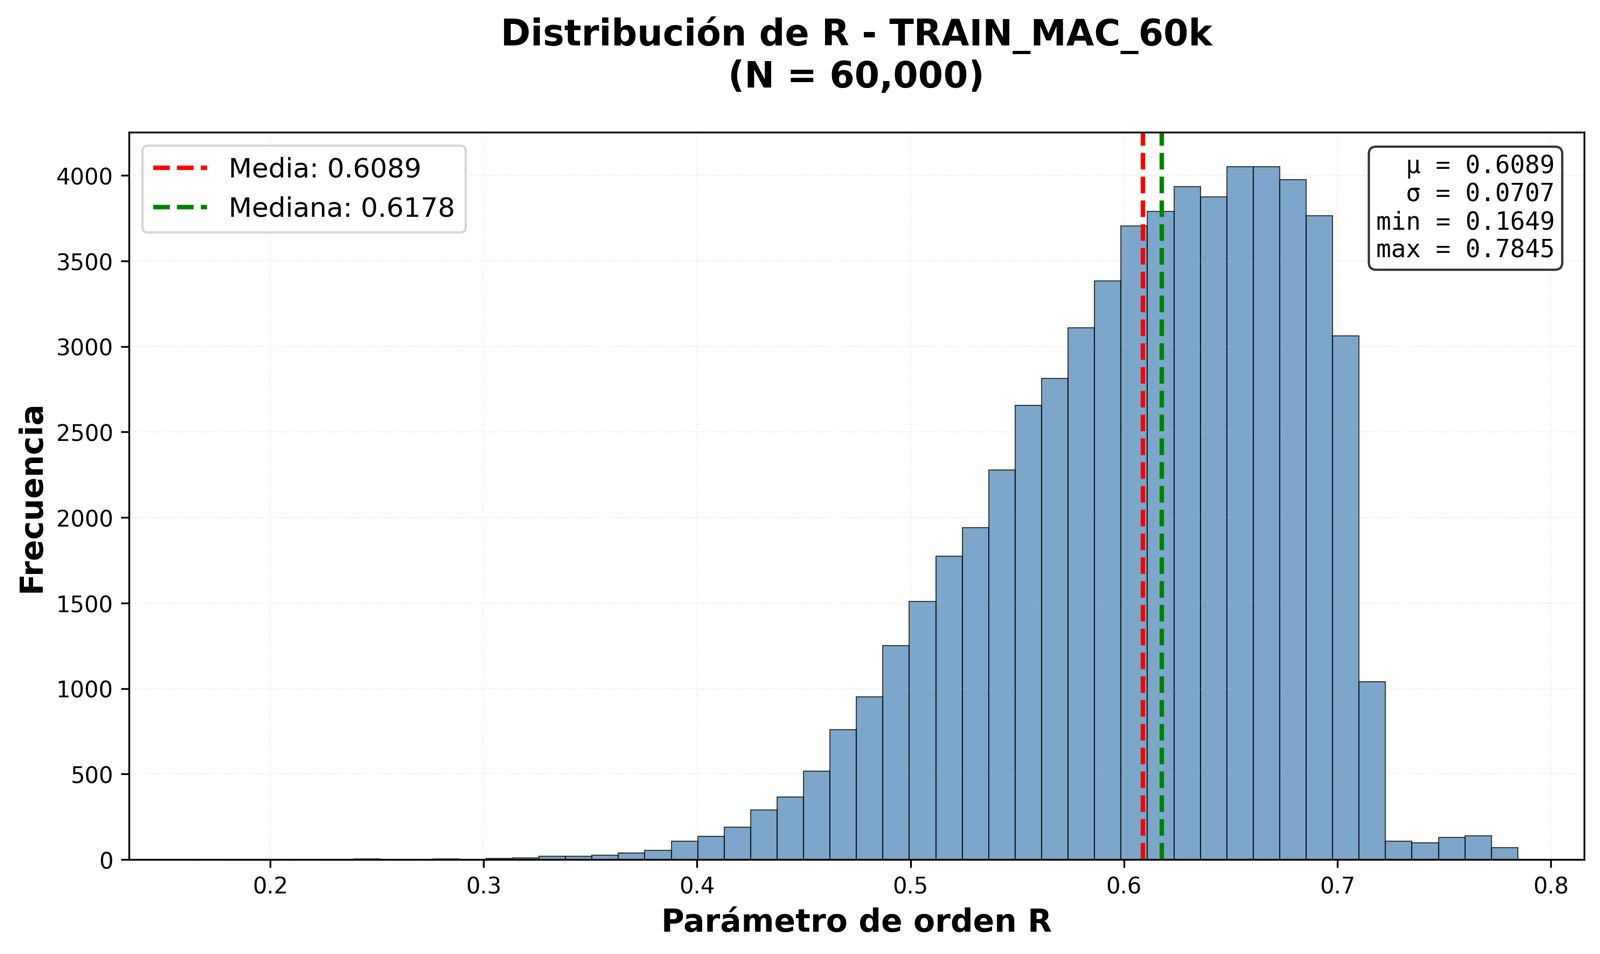
\includegraphics[width=0.8\linewidth]{rest.jpeg}
    \caption{Distribución del parámetro de orden estacionario para todo el data set.}
    \label{fig:rest}
\end{figure}

%Sincronización resultados
Se estudió la distribución del parámetro de orden estacionario para todo el conjunto de datos, cuyo resultado se muestra en la Figura~\ref{fig:rest}. En dicha figura se observa que la mayoría de los valores de $R$ se concentran en el intervalo entre 0.5 y 0.7, lo que indica que el sistema alcanza predominantemente un estado de sincronización parcial, mientras que solo un número reducido de configuraciones supera valores de $R > 0.7$. Asimismo, existe un subconjunto menor que alcanza el estado estacionario con valores inferiores a $R < 0.5$, lo que sugiere la posible presencia de dos regímenes dentro del sistema: uno dominante, caracterizado por sincronización parcial, y otro minoritario, asociado a configuraciones particulares que logran niveles más bajos de sincronización. Esta distribución evidencia una leve heterogeneidad en las dinámicas del sistema y apunta a que ciertas muestras presentan condiciones que limitan el grado de sincronización alcanzado. \\


Teniendo en cuenta la relación entre la variable $c$ que corresponde a la fuerza externa sobre la cual se orienta el sistema, y el parámetro de órden, se logra identificar una transición de fase de un estado desordenado a uno parcialmente ordenado. Esto se presenta como un ejemplo en la figura \ref{fig:ejemplo}. 

\begin{figure}[h!]
    \centering
    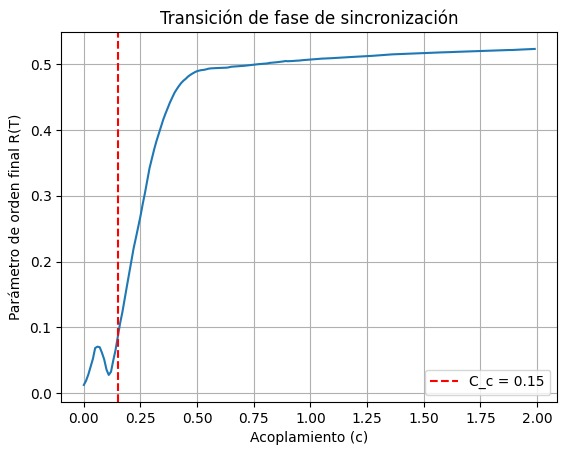
\includegraphics[width=0.5\linewidth]{cambio de fase.jpeg}
    \caption{Ejemplo de transición de fase para nuestro modelo utilizando una imagen del número 3 del data set MNIST}
    \label{fig:ejemplo}
\end{figure}

Para valores bajos de \(c\), el parámetro de orden final \(R(T)\) permanece cercano a cero y exhibe pequeñas fluctuaciones, lo que indica que el sistema se encuentra en un régimen desincronizado en el que la dinámica está dominada por variaciones iniciales y efectos numéricos. Al aproximarse al valor crítico \(c \approx 0.15\), marcado por la línea punteada, el comportamiento colectivo cambia abruptamente: el parámetro de orden comienza a aumentar de forma pronunciada, reflejando la aparición de sincronización global. En el intervalo \(0.15 < c < 0.5\), este crecimiento rápido caracteriza una transición de fase continua, típica de sistemas acoplados de tipo Kuramoto. Finalmente, para valores de acoplamiento mayores, la curva se estabiliza alrededor de \(R \approx 0.5\), indicando que el sistema alcanza un estado estacionario de sincronización parcial en el que incrementos adicionales del acoplamiento producen cambios marginales en el grado de coherencia global. \\


Teniendo en cuenta la figura anterior, entonces el $R$ crítico es aquel donde ocurre la transición de fase y así mismo para el $c$ crítico. Con esto, en la figura \ref{fig:distribución r crítico} se presenta la distribución de los $R$ críticos, por clase, es decir, por número. Estos datos se tomarón por separado para observar como se comportaba el sistema según las diferentes geometrías de los números.

\begin{figure}[h!]
    \centering
    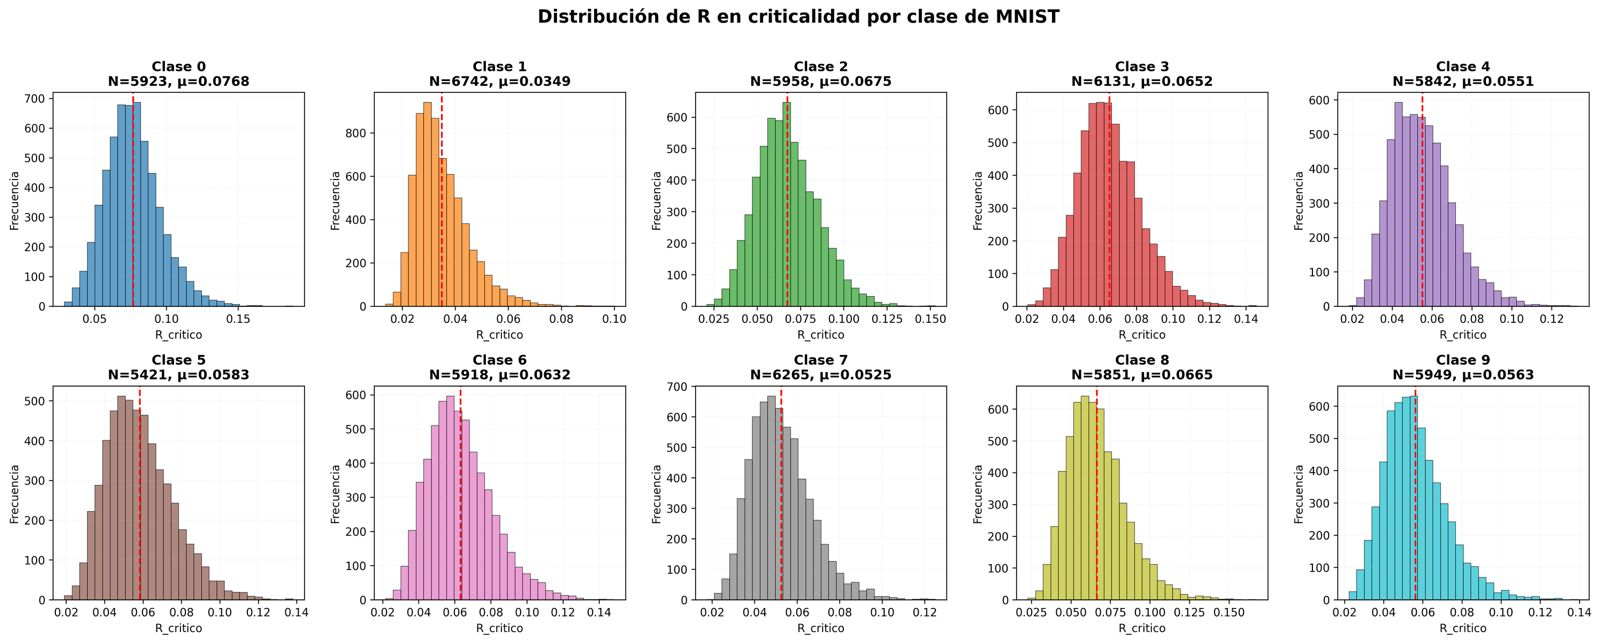
\includegraphics[width=1\linewidth]{distribución R crítico.jpeg}
    \caption{Caption}
    \label{fig:distribución r crítico}
\end{figure}

Las distribuciones del parámetro de orden crítico \(R_{\text{crítico}}\) para cada una de las diez clases del conjunto de datos MNIST. En todos los casos, las distribuciones son aproximadamente unimodales y presentan una ligera asimetría hacia la derecha, lo que indica que, aunque la mayoría de las muestras en cada clase alcanza valores relativamente bajos de sincronización en el punto crítico, existe un subconjunto reducido que logra valores más altos. Las medias de \(R_{\text{crítico}}\) se encuentran dentro de un rango estrecho, aproximadamente entre 0.035 y 0.07, lo cual sugiere que el comportamiento crítico del sistema es notablemente consistente entre clases y depende más de las propiedades globales del modelo que de las diferencias particulares entre dígitos. No obstante, se observan variaciones leves: las clases 0, 2 y 6 presentan valores medios ligeramente superiores, mientras que las clases 1 y 4 exhiben promedios menores, lo que podría estar asociado a diferencias en la complejidad geométrica o la distribución espacial de los trazos característicos de esas cifras. Además, el número de muestras por clase (del orden de 5800 a 6700) garantiza distribuciones estadísticamente robustas y comparables entre sí.\\


\begin{figure}[h!]
    \centering
    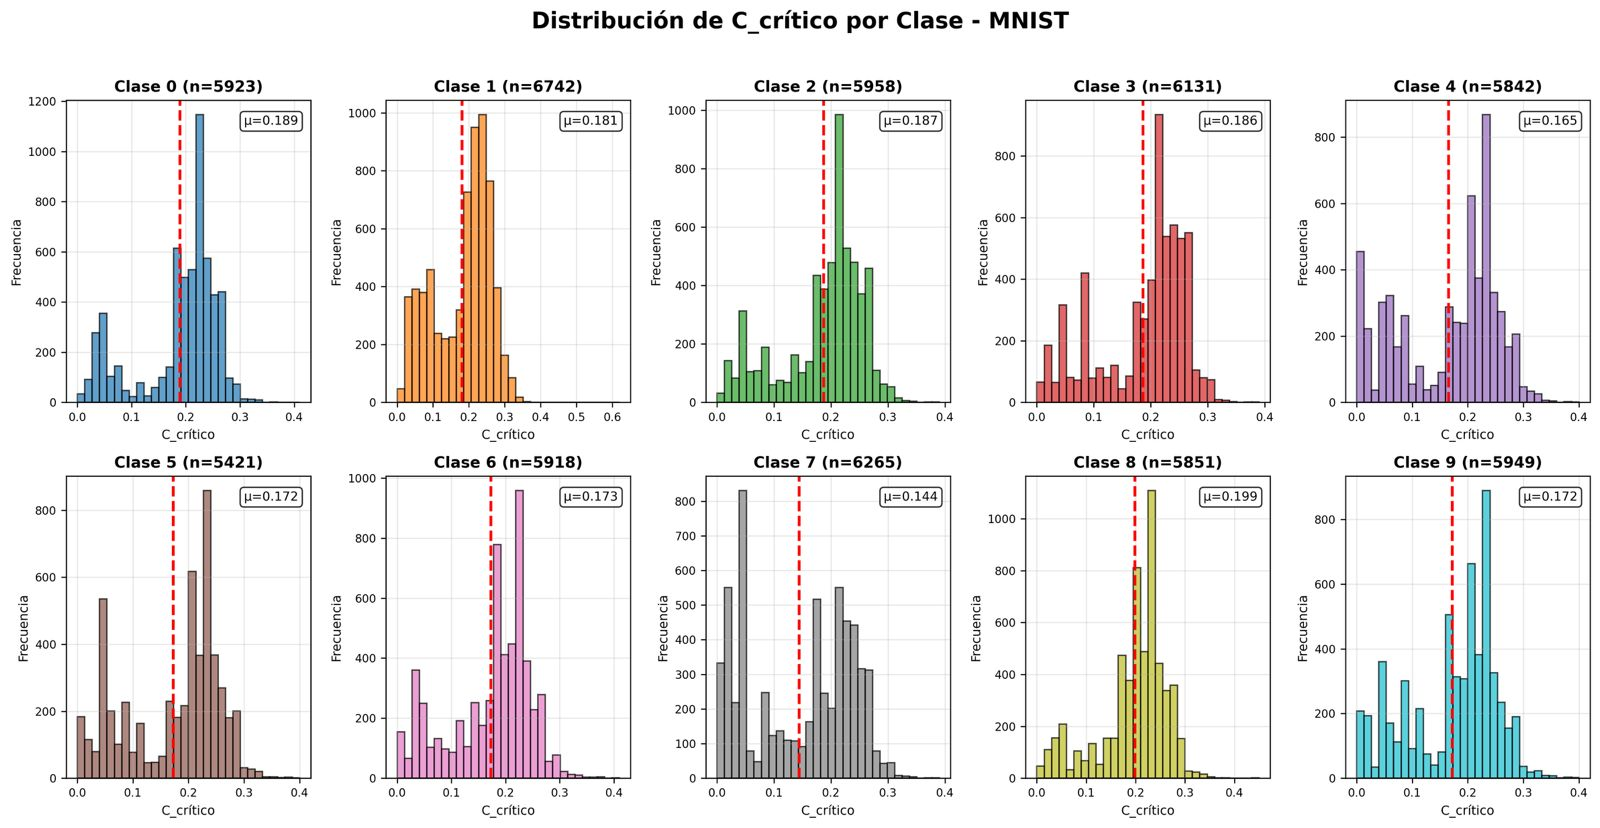
\includegraphics[width=1\linewidth]{distribución c crítico.jpeg}
    \caption{Caption}
    \label{fig:dis c critico}
\end{figure}


En la figura \ref{fig:dis c critico} las distribuciones de $C_{\text{crítico}}$ observadas para cada clase del conjunto MNIST se aprecia, de manera consistente, la presencia de dos grupos de valores que sugieren una estructura aparentemente bimodal. Este comportamiento indica que, aun dentro de una misma categoría de dígitos, existe una heterogeneidad significativa en la respuesta dinámica del sistema: algunas imágenes requieren un acoplamiento crítico menor para alcanzar la transición de sincronización, mientras que otras demandan valores considerablemente mayores. Esta separación en dos regímenes puede interpretarse como una consecuencia de variaciones morfológicas intraclase —como diferencias en trazo, forma, orientación o complejidad visual— que generan respuestas diferenciadas en la red de osciladores. En este sentido, la posible bimodalidad no constituye ruido estadístico, sino que revela la existencia de subpoblaciones estructurales dentro de cada clase, lo que sugiere que la dinámica de sincronización actúa de manera efectiva como un mecanismo de agrupamiento implícito sensible a las características internas de las imágenes.



\begin{figure}[h!]
    \centering
    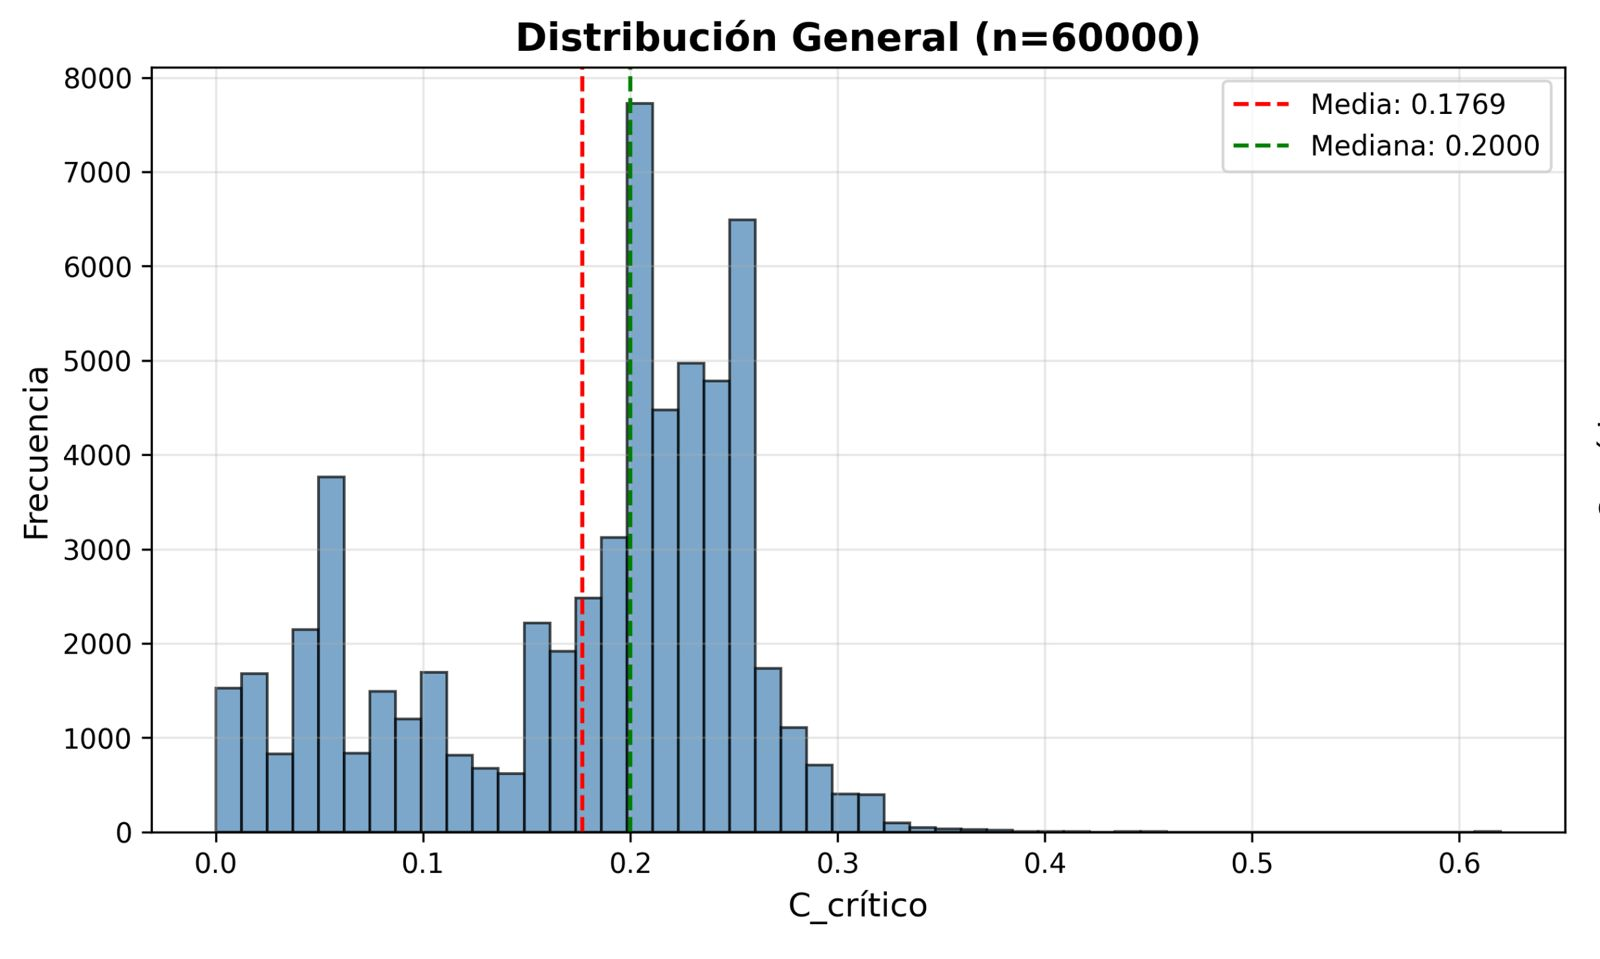
\includegraphics[width=0.5\linewidth]{distribución frecuencias c.jpeg}
    \caption{Caption}
    \label{fig:placeholder}
\end{figure}


%sincronización vs C (gráficas de distribuciones-----------------------------


\begin{figure}[h!]
    \centering
    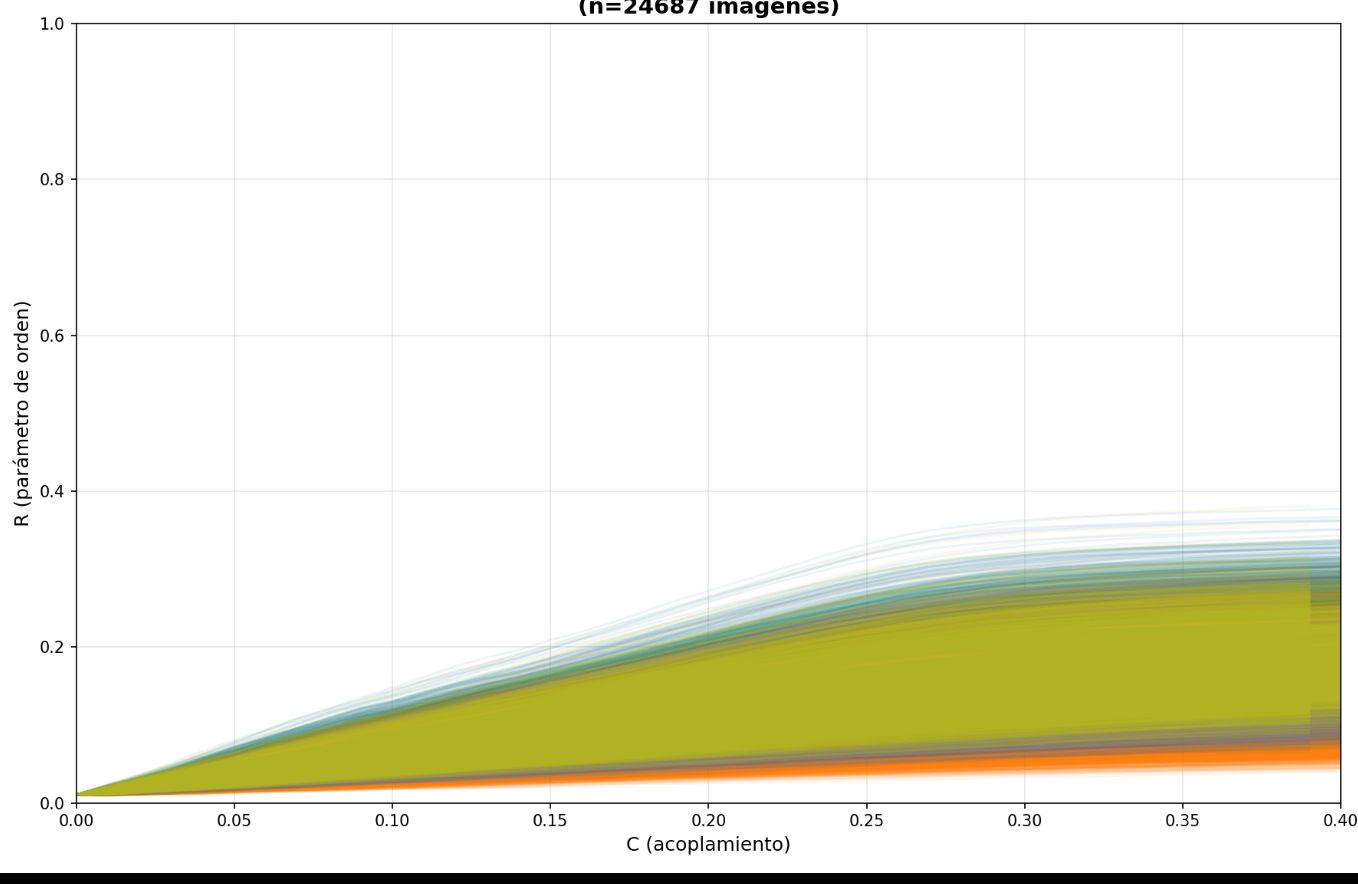
\includegraphics[width=0.7\linewidth]{parámetro vs c.jpeg}
    \caption{Caption}
    \label{fig:placeholder}
\end{figure}


\begin{figure}[h!]
    \centering
    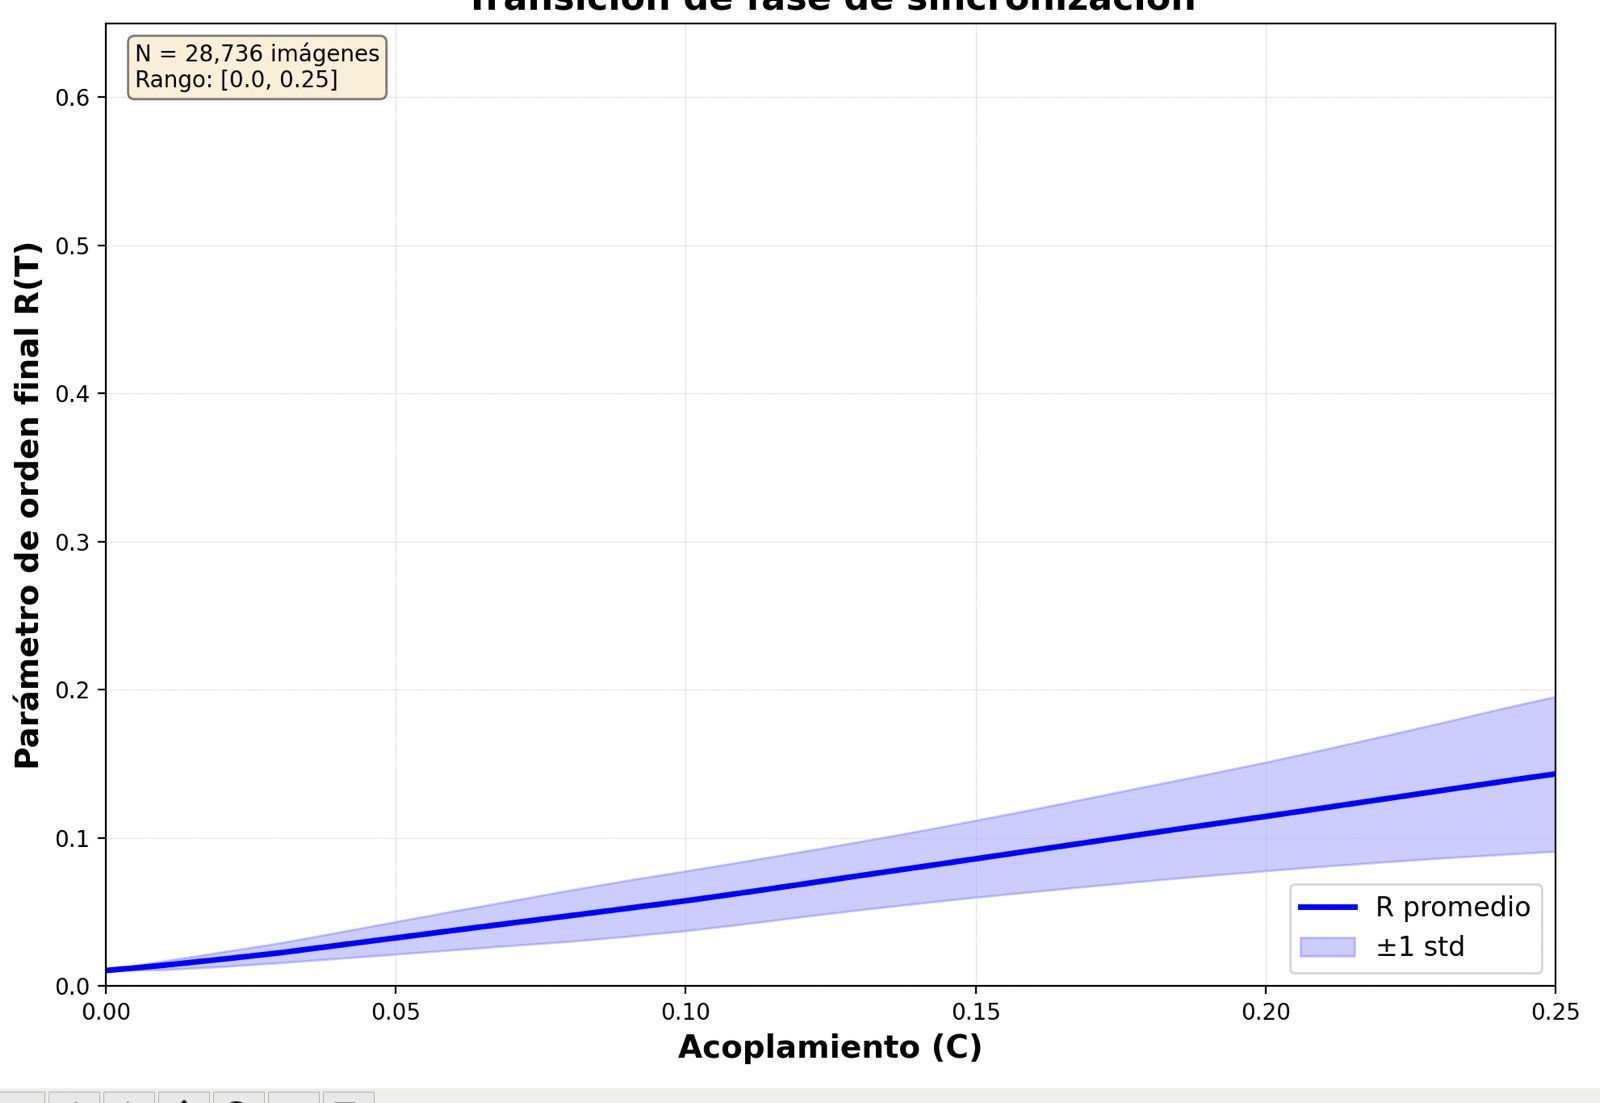
\includegraphics[width=0.7\linewidth]{promedio parametro vs c.jpeg}
    \caption{Caption}
    \label{fig:placeholder}
\end{figure}

%Entrenamiento de la red con los c

\begin{figure}[h!]
    \centering
    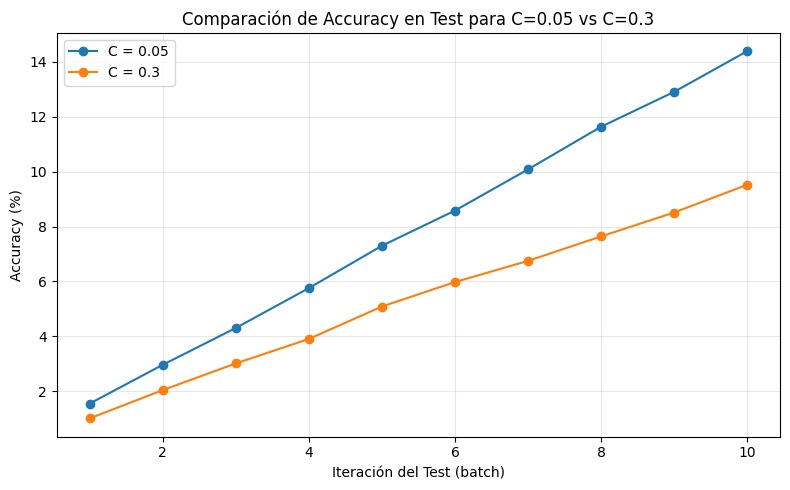
\includegraphics[width=0.7\linewidth]{comparación con loso C.jpeg}
    \caption{Caption}
    \label{fig:comparacion c}
\end{figure}



\section{Conclusiones}
\begin{itemize}
    \item MIYATO, Takeru, et al. Artificial Kuramoto Oscillatory Neurons. arXiv preprint arXiv:2410.13821, 2024.

    \item HIRST, Linda S. Fundamentals of soft matter science. CRC press, 2019.

    \item CHIALVO, Dante R. Emergent complex neural dynamics. Nature physics, 2010, vol. 6, no 10, p. 744-750.

    \item BETTINARDI, Ruggero G., et al. How structure sculpts function: unveiling the contribution of anatomical connectivity to the brain's spontaneous correlation structure. Chaos: An Interdisciplinary Journal of Nonlinear Science, 2017, vol. 27, no 4.

    \item SHANDILYA, Srinivas Gorur; TIMME, Marc. Inferring network topology from complex dynamics. New Journal of Physics, 2011, vol. 13, no 1, p. 013004.

    \item DE ARCANGELIS, Lucilla; HERRMANN, Hans J. Learning as a phenomenon occurring in a critical state. Proceedings of the National Academy of Sciences, 2010, vol. 107, no 9, p. 3977-3981.
\end{itemize}

\section{Bibliografía}
\begin{thebibliography}{99}
\bibitem{Kuramoto1984} Y. Kuramoto, \textit{Chemical Oscillations, Waves, and Turbulence}. Springer, 1984.
\bibitem{Strogatz2000} S. H. Strogatz, “From Kuramoto to Crawford: exploring the onset of synchronization in populations of coupled oscillators,” \textit{Physica D}, vol. 143, pp. 1–20, 2000.
\bibitem{Miyato2024} T. Miyato, \textit{et al.}, “Artificial Kuramoto Oscillatory Neurons (AKOrN),” arXiv:2410.13821, 2024.
\bibitem{Breakspear2010} M. Breakspear, S. Heitmann, and A. Daffertshofer, “Generative models of cortical oscillations: neurobiological implications of the Kuramoto model,” \textit{Frontiers in Human Neuroscience}, vol. 4, 2010.
\bibitem{ShewPlenz2013} W. L. Shew and D. Plenz, “The functional benefits of criticality in the cortex,” \textit{The Neuroscientist}, vol. 19, no. 1, pp. 88–100, 2013.
\bibitem{Myrov2024} V. Myrov, \textit{et al.}, “Hierarchical whole-brain modeling of critical synchronization dynamics in human brains,” bioRxiv 2024.05.08.593146, 2024.
\end{thebibliography}

\end{document}
